\newpage
\section{Grundlagen der Auswertung unstrukturierter Daten} \label{infos}
Siehe auch Wissenschaftliches Arbeiten~\footcite[\vglf][S. 1]{savic.2020}. %ohne textcommands
Damit sollten alle wichtigen Informationen abgedeckt sein ;-)~\footcite[\vglf][\pagef 1]{savic.2020} %mit textcommands
Hier gibt es noch ein Beispiel für ein direktes Zitat\footcite[][\pagef 1]{savic.2020} %mit textcommands

\subsection{Text Preprocessing}
Text Mining bezeichnet den Prozess, um wesentliche bekannte aber auch unbekannte Informationen aus Textdaten zu
generieren~\footcite[\vglf][\pagef 1]{mohan.2015}
Die Verarbeitung von unstrukturierten Textdaten wird auch als \ac{KDT}
bezeichnet und spielt eine signifikate Rolle in Anwendungsgebieten wie

\begin{itemize}
    \item Information Retrieval
    \item Information Extraction
    \item Natural Language Processing~\footcite[\vglf][\pagef 1 f.]{mohan.2015}
\end{itemize}
Im Wesentlichen geht es in allen \og Anwendungsgebieten um die Wissen durch das Mining der Texte zu generieren.

\begin{figure}[H]
    \caption{Text Mining Prozess}\label{fig:2_1_1_KDT_Process}
    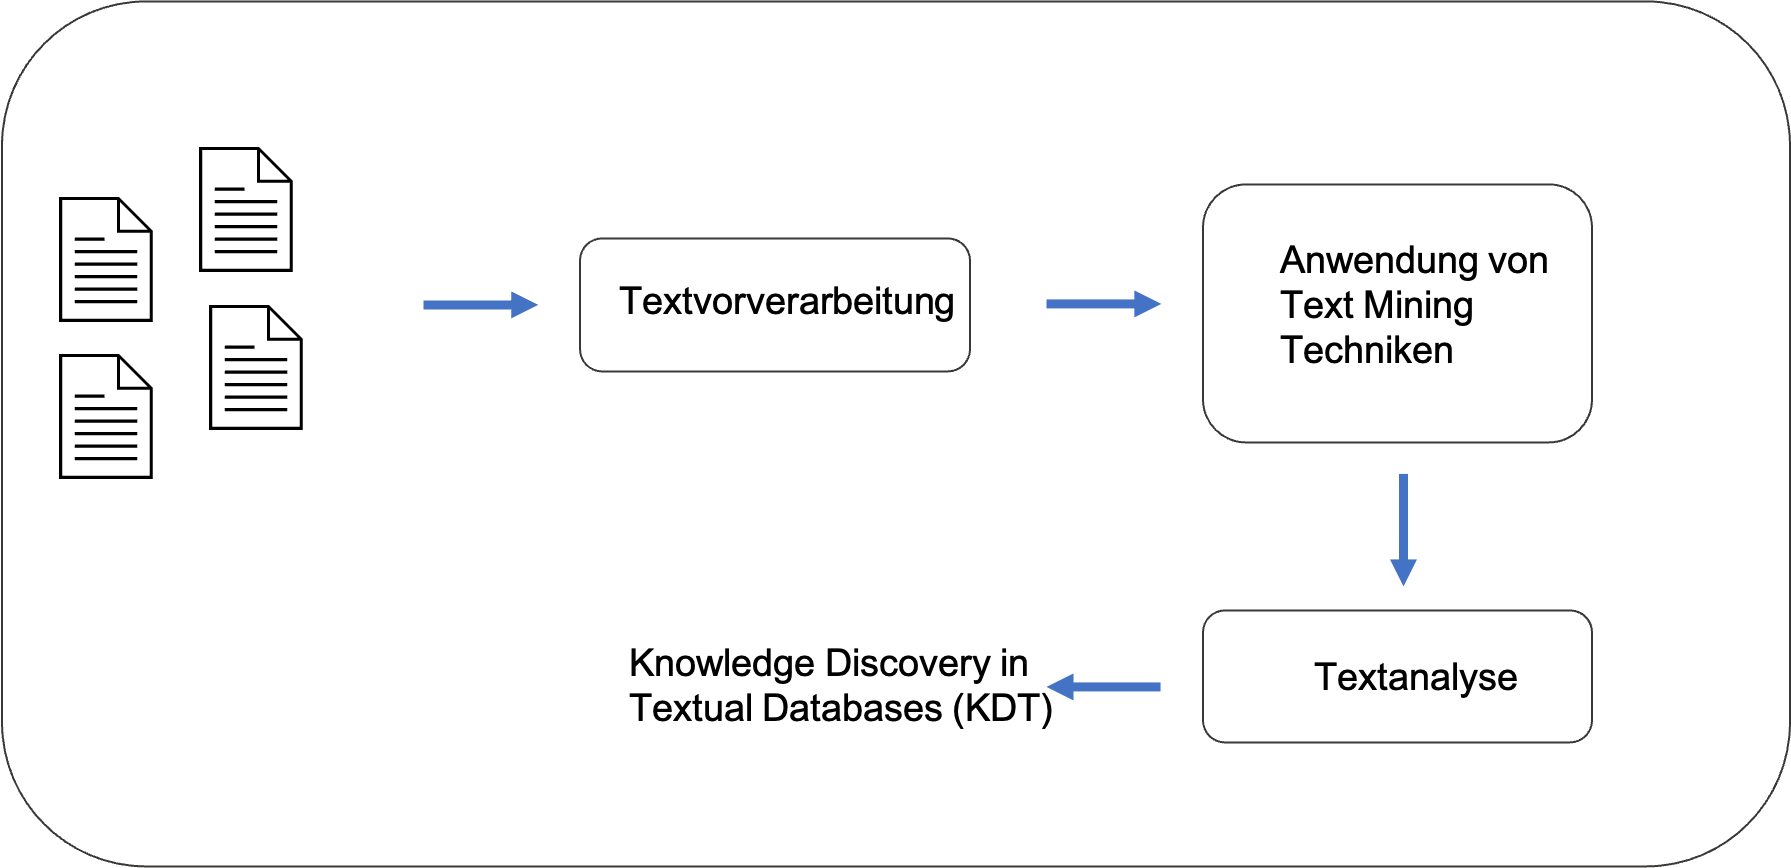
\includegraphics[width=0.9\textwidth]{2_1_1_KDT_Process}
    \\
    \textit{Quelle: Eigene Darstellung in Anlehnung an}~\cite[\pagef 1]{mohan.2015}
\end{figure}

Wie der Abbildung \ref{fig:2_1_1_KDT_Process} entnommen werden kann, stellt die Vorverarbeitung von Volltextdaten bei nahe
zu jeder Aufgabe im \ac{NLP} einen essentiellen und kritischen Schritt dar,
da hierbei die fundamentale Basis für die Weiterverarbeitung
sowie die Entwicklung der Modelle geschaffen wird.~\footcite[\vglf][\pagef 2]{gurusamy.2014}
Der Begriff der Textvorverarbeitung umfasst dabei die Anwendung unterschiedlicher Techniken/Methoden, bei
denen die Textdokumente für die eigentlichen Zielsetzungen vorbereitet werden.
Gängige Techniken für die Vorbereitung der Texte für die nachgelagerten Analysen können folgendermaßen aufgeteilt
werden:~\footcite[\vglf][\pagef 1]{pahwa.2018}

\begin{itemize}
    \item Inhalte Extrahieren und Bereinigen
    \item Annotationen
    \item Normalisieren
\end{itemize}

Zu Beginn der Volltextanalysen stehen häufig die Rohfassungen der Texte zur Verfügung. Diese gilt es im ersten
Schritt technisch einzulesen. Hierbei werden auch Daten mit eingelesen, dessen Informationsgehalt gering ist.
Beispielshaft zu nennen sind hier HTML tags, Werbung, etc beim Auslesen einer Website~\footcite[\vglf][\pagef 1]
{pahwa.2018} oder Grafiken, ASCII-Codes in PDF-Dateien. Demnach ist das Ziel bei dem \textbf{Extrahieren und Bereinigen
der Inhalte} die Rohdaten soweit zu säubern, bis sich schließlich die reinen Texte als Resultat ergeben.
Nachdem die Texte um die technischen Störfaktoren bereinigt wurden, ist die \textbf{Tokenization} eine typische Technik
der Textextraktion.
In dem Prozess der Tokenisation wird der gesamte zu analysierende Text in einzelne Wörter, Phrasen,
Symbole, etc. geteilt.
Hierbei wird das Ziel verfolgt die Bedeutung einzelner Wörter innerhalb eines Satzes zu analysieren.
Die Tokens dienen nämlich als Eingabewerte für viele weitergehende Prozessschritte.~\footcite[\vglf][\pagef 2]
{gurusamy.2014}
In jedem Text befinden sich Wörter, die wenig Informationsgehalt bei der Textanalyse bieten.
Solche Wörter werden auch als \textbf{Stop Words} bezeichnet.
Beispiele für solche Stop Words sind Artikel oder
Präpositionen wie \glqq{der}\grqq, \glqq{die}\grqq, \glqq{das}\grqq, \glqq{ein}\grqq,
\glqq{in}\grqq, \glqq{mit}\grqq, etc.
Im Analyseprozess stellt jedes unterschiedliche Wort eine eigene Dimension dar.
Durch die Entfernung der Stop Words wird somit die Dimensionshöhe reduziert bei gleichzeitiger Beibehaltung des
Informationsgehaltes des jeweiligen Satzes/Textes.~\footcite[\vglf][\pagef 3]{mohan.2015}\\
Neben der klassischen Methode, die Stop Words auf Basis einer vordefinierten Liste zu entfernen, sind diverse
mathematische und nicht-mathematische Methoden entwickelt worden, um Stop Words in Texten zu identifizieren und zu
bereinigen.\footnote{Detailiertere Informationen zu unterschiedlichen Methoden für die Entfernung von Stop Words
können \cite{mohan.2015} entnommen werden.}\\

\textcolor{red}{Annotationen: POS ergänzen!!!!}
Die Annotationen eines Textes sollen die Funktion des jeweiligen Wortes im Kontext des gesamten Satzes identifizieren.
\\


Bei dem \textbf{Normalisieren} von Texten wird das Ziel verfolgt ähnliche Wörter zu vereinheitlichen bzw.
diese auf einen Standard zu bringen.
Dieser Prozess soll vor allem die Dimensionen reduzieren, um die Berechnungen zu vereinfachen und gleichzeitig die
Effizienz durch die Standardiesierung der Wörter erhöhen.
\newline
Bei der Normalisierung von Wörtern wird häufig auf die Techniken des \textbf{Stemming} oder der \textbf{Lemmatization}
zurückgegriffen.
Das Stemming ist ein Prozess, der zugrundeliegende Wörter auf den Wortstamm herunterbricht.~\footcite[\vglf][\pagef 5]
{khyani.2021}
Dieser Wortstamm ist im Ergebnis häufig kein echtes Wort, sondern oftmals eine Buchstabenkombination bzw.
ein Präfix, den viele Wörter gemeinsam haben.~\footcite[\vglf][\pagef 5]{khyani.2021}
Es existiert eine Vielzahl an Stemming-Algorithmen, dessen Performance vom jeweiligen Einsatzbereich abhängt, sodass
noch kein Standard etabliert ist.\footnote{Eine ausführliche Analyse unterschiedlicher Stemming-Algorithmen kann
\cite{jivani.2011} entnommen werden.}
\newline
Die Idee bei der Lemmatization ist das so genannte \grqq{Lemma}\grqq{} oder auch die Vokabularform eines Wortes
zu identifizieren.~\footcite[\vglf][\pagef 7]{khyani.2021}
Der Prozess ist ähnlich dem des Stemmings, jedoch mit dem Unterschied im Ausgabewert.
Während beim Stemming der Ausgabewert der Wortstamm ist und oftmals kein echtes Wort,
ist der Ausgabewert bei der Lemmatization das Grundwort aus beispielsweise einem Wörterbuch.~\footcite[\vglf]
[\pagef 7]{khyani.2021}
Die Abbilung  \ref{fig:2_1_2_Stem_Lemma} verdeutlicht die Unterschiede der Lemmatization und des Stemmings anhand
des englischen Wortes \grqq{change}\grqq{} bzw. dessen Abwandlungen.

\begin{figure}[H]
    \caption{Stemming vs. Lemmatization}\label{fig:2_1_2_Stem_Lemma}
    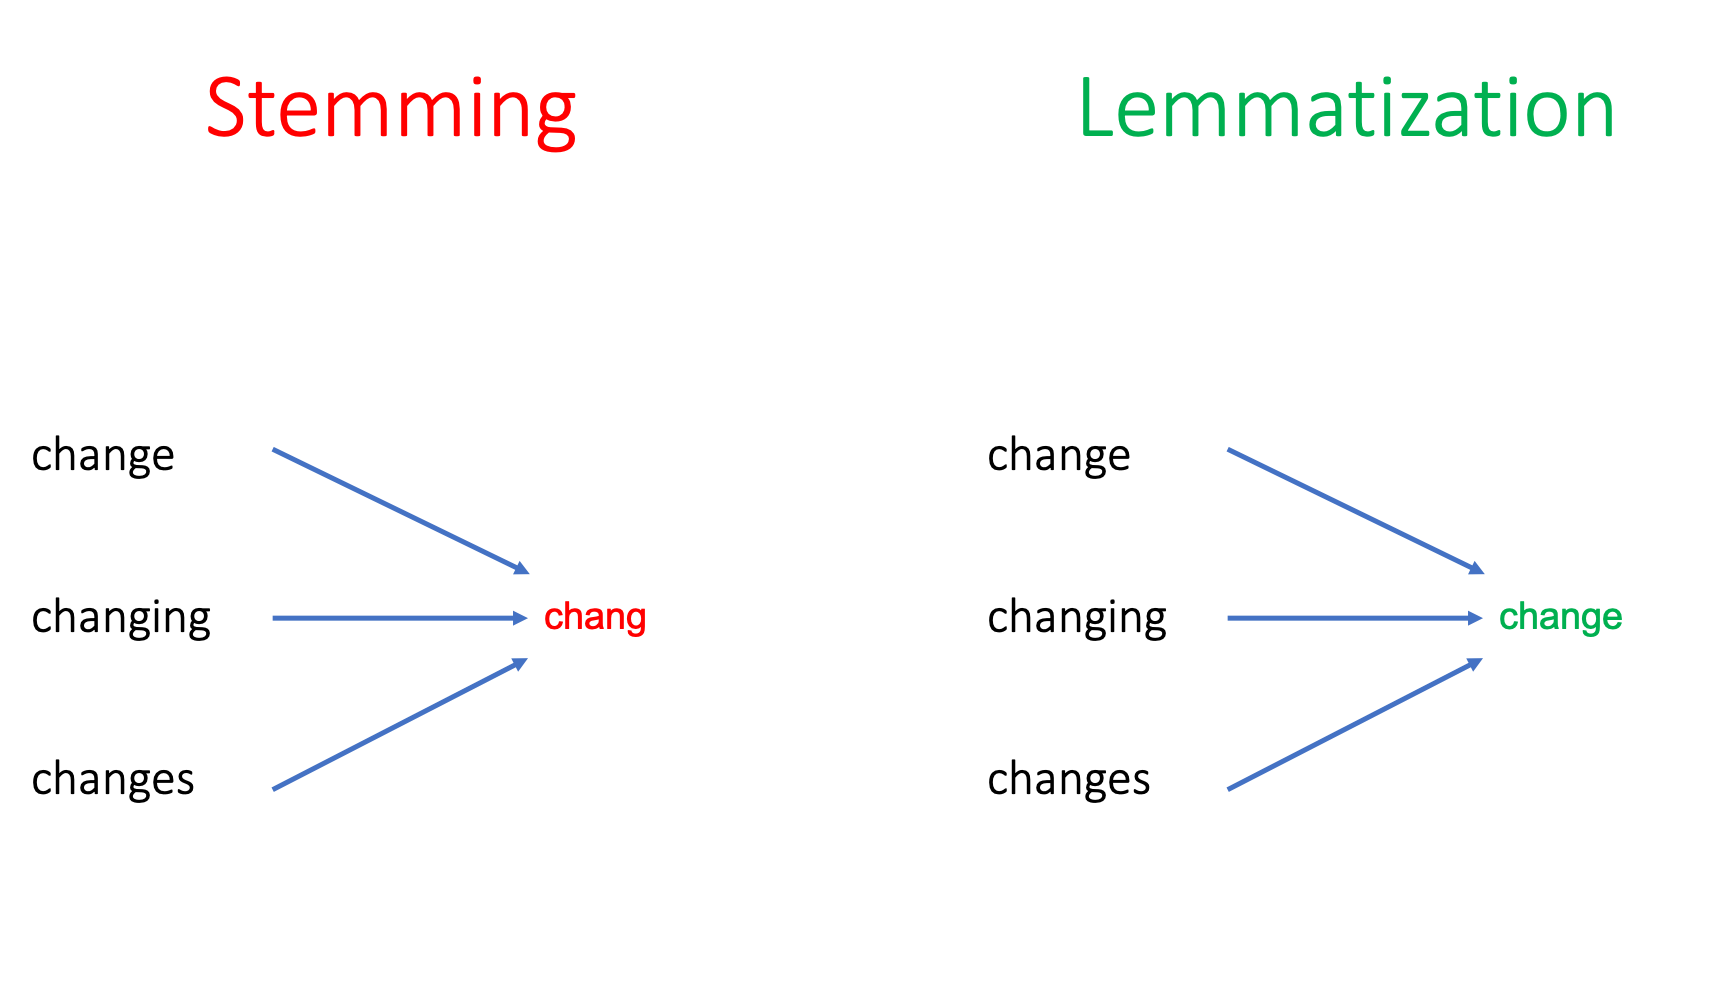
\includegraphics[width=0.9\textwidth]{2_1_2_Stem_Lemma}
    \\
    \textit{Quelle: Eigene Darstellung in Anlehnung an}~\cite[\pagef 7]{khyani.2021}
\end{figure}


\subsection{Named Entity Recognition}

\begin{itemize}
    \item Was ist NER
    \item Wie kommen wir an Daten und Tools?
    \item Was sind NER-Möglichkeiten - Klassische NER / DL-NER)
\end{itemize}

\subsection{Named Entity Linking}